\documentclass[11pt]{article}
\usepackage[utf8]{inputenc}
\usepackage[T1]{fontenc}
\usepackage{lmodern}
\usepackage[margin=1in]{geometry}
\usepackage{amsmath,amssymb,amsthm}
\usepackage{enumitem}
\usepackage{booktabs}
\usepackage{xcolor}
\usepackage{tikz}
\usepackage[colorlinks=true,bookmarks=false,linkcolor=blue!50!black,urlcolor=blue!50!black]{hyperref}

\theoremstyle{plain}
\newtheorem{theorem}{Theorem}
\newtheorem{lemma}[theorem]{Lemma}
\newtheorem{claim}[theorem]{Claim}
\newtheorem{corollary}[theorem]{Corollary}
\theoremstyle{definition}
\newtheorem{definition}[theorem]{Definition}
\newtheorem{example}[theorem]{Example}
\theoremstyle{remark}
\newtheorem*{remark}{Remark}

\newcommand{\N}{\mathbb{N}}
\newcommand{\Z}{\mathbb{Z}}
\newcommand{\R}{\mathbb{R}}
\newcommand{\Q}{\mathbb{Q}}
\newcommand{\iv}[1]{[#1]}                 % Iverson bracket
\newcommand{\powerset}{\mathcal{P}}
\DeclareMathOperator{\ord}{ord}
\DeclareMathOperator{\gcdop}{gcd}

\setlength{\parindent}{0pt}
\setlength{\parskip}{0.6em}
\newcommand{\lesson}[2]{\href{../lessons/#1}{#2}}   % link to a lesson image

% Let long inline lists like \{1,2,5,6\} break across lines after a comma.
\mathchardef\mycomma="613B
\mathcode`,="8000
{\catcode`,=\active \gdef,{\mycomma\penalty0\hspace{0pt}}}
\emergencystretch=2em

\newcommand{\blue}{\text{blue}}
\newcommand{\red}{\text{red}}
\title{Ramsey theory: $R(3,3)=6$, Ramsey's theorem,\\ the binomial bound, $R(4,4)=18$}
\author{Notes from Carlos' lessons}
\date{}
\begin{document}
\maketitle

\textbf{Source lessons (chronological):}
\lesson{2026-02-27-ramsey-numbers.png}{02-27},
\lesson{2026-03-01-ramsey-theorem.png}{03-01},
\lesson{2026-03-06-ramsey-numbers-bounds-4-4.png}{03-06},
\lesson{2026-04-10-ramsey-numbers-r44-is-18.png}{04-10} (and \lesson{2026-04-10-ramsey-numbers-r44-is-18-alt.png}{alt}),
\lesson{2026-04-16-ramsey-numbers-r44-is-18.png}{04-16} (and \lesson{2026-04-16-ramsey-numbers-r44-is-18-alt.png}{alt}).
Code: \texttt{../code/ramsey-4-4.py}.

\medskip
\textbf{Setup.} Colour the edges of the complete graph $K_N$ with two colours. $R(r,s)$ is the least $N$ such that every colouring has a red $K_r$ or a blue $K_s$. (The 02-27 board uses green/purple and writes $R(n,m)$.) Immediate facts: $R(r,s)=R(s,r)$ (swap the colours), and $R(r,2)=r$ (either some edge is blue, or all edges are red and form a red $K_r$).

\section{$R(3,3)=6$}

\paragraph{Lower bound, $R(3,3)>5$.} Colour $K_5$ with a red $5$-cycle (the outer pentagon) and a blue $5$-cycle (the pentagram). Neither colour contains a triangle. This is the $5$-vertex picture on the 02-27 and 03-01 boards.

\begin{center}
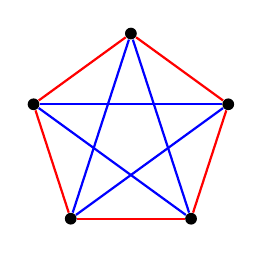
\begin{tikzpicture}[scale=1.3,every node/.style={circle,fill=black,inner sep=1.5pt}]
  \foreach \i in {0,...,4} \node (v\i) at ({90+72*\i}:1) {};
  \foreach \i/\j in {0/1,1/2,2/3,3/4,4/0} \draw[red,thick] (v\i)--(v\j);
  \foreach \i/\j in {0/2,2/4,4/1,1/3,3/0} \draw[blue,thick] (v\i)--(v\j);
\end{tikzpicture}
\end{center}

\paragraph{Upper bound, $R(3,3)\le6$.} Take any colouring of $K_6$ and a vertex $v$. Its $5$ edges have two colours, so at least $3$ have the same colour, say red to $a,b,c$. If any of $ab,bc,ac$ is red, it forms a red triangle with $v$. Otherwise $abc$ is a blue triangle. \qed

\paragraph{The double-counting attempt on the 02-27 board (my reading).} The board counts, for $K_6$, the purple edges $P$ and green edges $G$ via triangles. Each edge lies in $4$ triangles, so $4P=\sum_{\triangle}P(\triangle)$ and $4G=\sum_{\triangle}G(\triangle)$, and $P(\triangle)+G(\triangle)=3$ gives $4(P+G)=3\binom63=60$, i.e.\ $P+G=15$. If there were no monochromatic triangle, each triangle would have $1$ or $2$ purple edges, so $20\le4P\le40$, i.e.\ $5\le P,G\le10$. That is consistent with $P+G=15$, so this count alone does \emph{not} give a contradiction; the pigeonhole argument above is the one that proves $R(3,3)\le6$. (The handwriting is faint; the numbers $15$, $20\le4P\le40$, $5\le P\le10$ are legible.)

\section{Ramsey's theorem: $R(r,s)$ exists}

\begin{theorem}[Ramsey]
For all $r,s\ge2$, $R(r,s)$ exists.
\end{theorem}
\begin{proof}
Induction on $r+s$ (the board's hypothesis $Q(N)$). Base: $R(r,2)=r$ and $R(2,s)=s$ exist; in particular $R(2,2)=2$ (the case $r+s=4$).

Step: assume $R(r-1,s)$ and $R(r,s-1)$ exist. We claim $R(r,s)\le R(r-1,s)+R(r,s-1)$.

Take a colouring of $K_N$ with $N=R(r-1,s)+R(r,s-1)$ and a vertex $v$. Let $R_v$ be its red neighbours and $B_v$ its blue neighbours, so $|R_v|+|B_v|=N-1=R(r-1,s)+R(r,s-1)-1$. If both $|R_v|\le R(r-1,s)-1$ and $|B_v|\le R(r,s-1)-1$, the sum would be at most $N-2$. So either $|R_v|\ge R(r-1,s)$ or $|B_v|\ge R(r,s-1)$.
\begin{itemize}[nosep]
  \item \emph{Case $|R_v|\ge R(r-1,s)$.} Inside $R_v$ there is a red $K_{r-1}$ or a blue $K_s$. A red $K_{r-1}$ together with $v$ is a red $K_r$.
  \item \emph{Case $|B_v|\ge R(r,s-1)$.} Symmetric: a blue $K_{s-1}$ together with $v$ is a blue $K_s$, or $B_v$ already holds a red $K_r$.
\end{itemize}
Either way the colouring contains a red $K_r$ or a blue $K_s$.
\end{proof}

\section{The explicit bound $R(r,s)\le\binom{r+s-2}{r-1}$}

The 03-01 board turns the inequality into the recurrence $U(r,2)=r$, $U(2,s)=s$, $U(r,s)=U(r-1,s)+U(r,s-1)$, so $R(r,s)\le U(r,s)$ by induction. The 03-06 board solves it with Pascal's identity.

\begin{theorem}
$R(r,s)\le\dbinom{r+s-2}{r-1}$.
\end{theorem}
\begin{proof}
Induction on $r+s$. Base: $\binom{r}{r-1}=r$ and $\binom{s}{1}=s$. Step:
\[
R(r,s)\le R(r-1,s)+R(r,s-1)\le\binom{r+s-3}{r-2}+\binom{r+s-3}{r-1}=\binom{r+s-2}{r-1}.
\]
\end{proof}

Sample consequences: $R(3,3)\le\binom42=6$ and $R(4,4)\le\binom63=20$ (the board also tabulates the binomials in a grid). It also lists $43\le R(5,5)\le46$; further bounds for $R(6,6)$ and $R(10,10)$ are on that board, but the handwriting is too small for me to transcribe them reliably.

\section{$R(4,4)=18$}

Notation on the 04-10 board: ``$n\to(b,r)$'' means every colouring of $K_n$ (blue/red) has a blue $K_b$ or a red $K_r$; so $R(b,r)$ is the least such $n$. Known: $6\to(3,3)$ and $4\to(2,4)$.

\subsection{Upper bound: $18\to(4,4)$}

\begin{lemma}[Parity improvement]
Let $n_1\to(b,r-1)$ and $n_2\to(b-1,r)$. Then $n_1+n_2\to(b,r)$; and if $n_1,n_2$ are both even, already $n_1+n_2-1\to(b,r)$.
\end{lemma}
\begin{proof}
Take a colouring of $K_N$ with $N=n_1+n_2-1$ (the weaker claim with $N=n_1+n_2$ is the argument of Section~2). Each vertex $v$ has $N-1=n_1+n_2-2$ neighbours.
\begin{itemize}[nosep]
  \item If $\deg_R(v)\ge n_1$: the red neighbourhood has $\ge n_1\to(b,r-1)$ vertices, so it contains a blue $K_b$ (done) or a red $K_{r-1}$ (add $v$ to get a red $K_r$).
  \item If $\deg_B(v)\ge n_2$: symmetrically, a blue $K_{b-1}$ plus $v$ is a blue $K_b$, or a red $K_r$ appears.
\end{itemize}
So if the colouring has no blue $K_b$ and no red $K_r$, no vertex satisfies either condition: $\deg_R(v)\le n_1-1$ and $\deg_B(v)\le n_2-1$ for all $v$. Their sum is $n_1+n_2-2$, so both are equalities: $\deg_R(v)=n_1-1$ for every $v$. If $n_1$ is even, $n_1-1$ is \textbf{odd}, and $N=n_1+n_2-1$ is odd. So the graph has an odd number of vertices, each with odd red degree, and $\sum_v\deg_R(v)$ is odd. But by the handshake lemma it equals $2|E_R|$, which is even. Contradiction.
\end{proof}

\paragraph{Applications.}
\begin{itemize}[nosep]
  \item $R(3,4)\le9$: take $b=3$, $r=4$, $n_1=R(3,3)=6$, $n_2=R(2,4)=4$, both even, so $6+4-1=9$. (Known: $R(3,4)=9$.)
  \item $R(4,4)\le R(4,3)+R(3,4)=9+9=18$.
\end{itemize}

\subsection{Lower bound: $17\not\to(4,4)$ (the Paley graph on $\Z_{17}$)}

Vertices $0,1,\dots,16$. Let $Q=\{x^2\bmod17\}=\{1,2,4,8,9,13,15,16\}$ be the non-zero quadratic residues (the squares $1,4,9,16,25\equiv8,36\equiv2,49\equiv15,64\equiv13$). Colour $\{x,y\}$ red if $x-y\in Q$ and blue otherwise. This is well defined because $-1\equiv4^2\in Q$ (the board checks $x>y$ and $x-y\in\{1,2,4,8,9,13,15,16\}$). Each vertex has red degree $8$ and blue degree $8$.

\paragraph{Facts about $Q$.} Take the primitive root $g=3$, so $\Z_{17}^\times=\{g^0,\dots,g^{15}\}$ and $g^{16}=1$. Then $Q$ is exactly the set of even powers of $g$. Indeed $(g^t)^2=g^{2t}$ is even; conversely, if $g^m=(g^t)^2$ with $m$ odd, then $g^{m-2t}=1$ forces $16\mid m-2t$, impossible by parity. Hence, writing $N$ for the non-residues (the odd powers):
\begin{itemize}[nosep]
  \item $Q\cdot Q=Q$, $N\cdot N=Q$, $Q\cdot N=N$, as in the board's multiplication table.
  \item \textbf{Symmetry.} Multiplying all vertices by $q\in Q$ maps red edges to red edges (since $q(x-y)\in Q\iff x-y\in Q$); multiplying by a non-residue swaps the colours. So the graph is isomorphic to its complement, and translations $x\mapsto x+r$ are also symmetries.
\end{itemize}

\paragraph{No red $K_4$.} Suppose $\{a,b,c,d\}$ is a red $K_4$. Translate by $-a$ and scale by $(b-a)^{-1}\in Q$ (allowed because $b-a\in Q$): we may assume the clique is $\{0,1,p,q\}$. Red edges to $0$ and to $1$ require $p,q\in Q$ and $p-1,q-1\in Q$. Checking $Q$:

\begin{center}
\begin{tabular}{@{}lcccccccc@{}}
\toprule
$p\in Q$ & 1 & 2 & 4 & 8 & 9 & 13 & 15 & 16\\
$p-1\in Q$? & no ($0$) & yes & no ($3$) & no ($7$) & yes & no ($12$) & no ($14$) & yes\\
\bottomrule
\end{tabular}
\end{center}

So $p,q\in\{2,9,16\}$ (the board boxes exactly these three). But $2-9\equiv10$, $2-16\equiv3$, $9-16\equiv10$, and none is in $Q$, so no two of them are red-adjacent. Contradiction. (Also checked by brute force over all $\binom{17}{4}$ subsets.)

\paragraph{No blue $K_4$.} Multiplication by a non-residue (say $3$) maps a blue $K_4$ to a red $K_4$. \qed

So $R(4,4)\ge18$, and with the upper bound, $R(4,4)=18$.

\section*{Notes}
\begin{itemize}[nosep]
  \item The ``theory-builders vs.\ problem-solvers'' remark in the top-right of the 03-06 board (Euler/Gauss/Grothendieck vs.\ Erd\H{o}s) and the van der Waerden question beside it are asides; the latter is picked up in the topic \emph{Van der Waerden's theorem}.
  \item The \texttt{-alt} images are slightly different exports of the 04-10 and 04-16 boards with the same content.
  \item Greenwood--Gleason (1955) first showed the $17$-vertex lower bound; see \href{https://plus.maths.org/proving-r4417}{Proving that $R(4,4)>17$ (Plus Magazine)}. The web sources I found did not spell out the parity argument for the upper bound, so the lemma above is my write-up of what the 04-10 board sketches (its labels: $n_1\to(b,r-1)$, $n_2\to(b-1,r)$, odd/even degrees, ``$\sum\deg v=2|E|$ even!'').
\end{itemize}

\end{document}
